\documentclass{article}
\usepackage{amsmath}
\usepackage[utf8]{inputenc}
\usepackage{graphicx}
\usepackage{braket}
\usepackage{dcolumn}
\usepackage{amsfonts}
\usepackage{amssymb}
\usepackage{bm}
%\usepackage{showkeys}
\usepackage{ragged2e}
\usepackage{cite}
\usepackage{authblk}
\usepackage{xcolor}
\newif{\ifmover}
\newif{\ifquitar}
\renewcommand{\Affilfont}{\small}
\newcommand{\notaL}[1]{{\color{orange}L: #1}}
\newcommand{\notaVA}[1]{{\color{orange}VA: #1}}
\newcommand{\notaVCG}[1]{{\bf \em \color{orange}VCG: #1}}
\definecolor{Addtext}{RGB}{0,0,255}
\begin{document}

	%\title{Thickness optimization in wide range quasi omnidirectional multilayer
	% structures}
	\title{Suplementary information: Optimization of wide-band
          quasi-omnidirectional 1-D photonic structures}
	\author[1,2,3]{Victor Castillo-Gallardo\thanks{email: {\tt
				victor1\_1@hotmail.com}}}
	\author[1,2,3]{Luis Eduardo Puente-Díaz}
	\author[4]{D. Ariza-Flores}
	\author[3]{Hector Pérez-Aguilar}
	\author[2]{W. Luis Mochán\thanks{email: {\tt
				mochan@fis.unam.mx}}}
	\author[1]{Vivechana Agarwal\thanks{email: {\tt
				vagarwal@uaem.mx}}}
	\affil[1]{Centro de Investigación en Ingeniería y Ciencias Aplicadas,
		Universidad del Estado de Morelos, Av. Universidad 1001
		Col. Chamilpa, Cuernavaca, Morelos 62209, México.}
	\affil[2]{Instituto de Ciencias Físicas, Universidad Nacional Autónoma
		de México, Av. Universidad S/N, Col. Chamilpa, 62210 Cuernavaca,
		Morelos, México.}
	\affil[3]{Facultad de Ciencias Físico Matemáticas,
		Universidad Michoacana de San Nicolás de Hidalgo, Av. Francisco
		J. Múgica S/N 58030, Morelia, Mich., México.}
	\affil[4]{Conacyt-Universidad Autónoma de San Luis Potosí, Karakorum 1470, Lomas 4ta Secc, San Luis Potosí, S.L.P., 78210, México.}
	%\date{{\small {\today}}}
	\maketitle

\section{Development of the transfer matrix}

Consider a system that varies along  the $z$ axis only, as show in Fig.
\ref{Fig1}(a). Its transfer matrix $\bm{M}(z_{2},z_{1})$
is a
2x2 matrix that relates the components  $E_{\parallel }$ and
$H_{\parallel }$ of the electric and magnetic fields parallel to the $xy$ plane and
normal to the axis of the structure, evaluated at any two points $z_{2}$
and $z_{1}$,
\begin{equation*}
\left(
\begin{array}{c}
E_{\Vert } \\
H_{\Vert }%
\end{array}%
\right) _{z_{2}}=\bm M( z_{2},z_{1}) \left(
\begin{array}{c}
E_{\Vert } \\
H_{\Vert }%
\end{array}%
\right) _{z_{1}}.
\end{equation*}%

Many equivalent formulations have been proposed to obtain $\bm M$. For
a periodically
replicated multilayered system, the transfer matrix may be constructed
from the normal modes of the corresponding photonic crystal. These
modes are described by Bloch's
theorem, which reads in this case,
\begin{equation}
\begin{pmatrix}
E_{\Vert }^{\pm } \\
H_{\Vert }^{\pm }%
\end{pmatrix}%
_{z_{N}}=\bm M%
\begin{pmatrix}
E_{\Vert }^{\pm } \\
H_{\Vert }^{\pm }%
\end{pmatrix}%
_{z_{0}}=e^{\pm iKD}%
\begin{pmatrix}
E_{\Vert }^{\pm } \\
H_{\Vert }^{\pm }%
\end{pmatrix}%
_{z_{0}},  \label{Bloch}
\end{equation}%
where $D=z_{N}-z_{0}$ is the period, which corresponds to the actual
thickness of the multilayered system, and $\pm K$ is the 1D Bloch's
vector describing the propagation along $z$. Thus, $\Lambda_{\pm }=e^{\pm iKD}$ are
the eigenvalues of transfer matrix $\bm M$ and $E_{\Vert }^{\pm }$ and $H_{\Vert
}^{\pm }$ are the corresponding eigenvectors. Notice that $\det M=1$  exactly,
so the product of eigenvalues $\Lambda_{+}\Lambda_{-}=1$ and the
dispersion relation of the Bloch modes becomes
\begin{equation}
\cos KD=\frac{1}{2}\text{Tr}\,\bm M  \label{dispersion}
\end{equation}%
where T$\text{r}$ denotes the trace. \begin{figure}[tbph]
	\begin{center}
		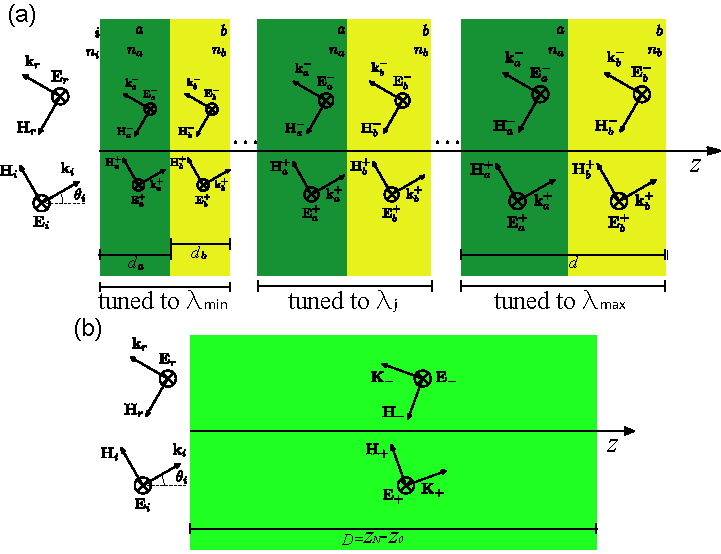
\includegraphics[width=\textwidth]
		{SIF1Squeme1DPC.pdf}
	\end{center}
	\caption{(a) Chirped-type photonic structure formed by two alternating
		materials $a$ and $b$, with refractive indices $n_{a}$ and $n_{b}$,
		thickness $d_{a}$ and $d_{b}$ that increases gradually
                according to some design scheme. We show schematically
                the  incident and reflected electric and magnetic
                fields, $\bm E_i$, $\bm H_i$,  $\bm E_r$, $\bm H_r$,
                their wavevectors $\bm k_i$ and $\bm k_r$, the right
                ($+$) and left ($-$) moving fields within each layer
                as well as their wavevectors $\bm k_\alpha^\pm$. (b)
                The multilayer system can be replaced by an
		effective layer within which supports right and left
                moving Bloch waves with wavevectors $\bm K^\pm=(\bm Q,
                \pm K)$ and electric and magnetic field amplitudes
                $\bm E_\beta^\pm$ and $\bm H_\beta$. The projection of
              the wavevector unto the $xy$ plane is $\bm Q$ for all
              the waves, due to translational symmetry and $K$ is
              obtained from Eq. \eqref{dispersion}.}
	\label{Fig1}
\end{figure}

Now, consider a finite system made of $P$ periods, with thickness $PD$
and placed on a substrate. Even for the extreme $P=1$  case, the
optical properties of this system can be obtained by considering an incoming
wave from the ambient, a wave reflected to the environment, a wave
transmitted to the substrate, and two Bloch waves within the structure, one
moving rightwards and other leftwards, as show in Fig. \ref{Fig1}(b). Hence, the
continuity of $E_{\Vert }$ and $H_{\Vert }$ yields two
equations at each interface, with which the four unknowns are obtained,
namely the reflection and transmission amplitudes $r$ and $t$, and the
amplitudes of the two Bloch's waves. In a finite system,
$K$ can be complex. Even in the presence of very little dissipation, Bloch's
waves should decay as they propagate. Thus, the eigenvalue of the right-moving mode
$\Lambda_{+}=e^{iKD}$ is identified as the one that obeys
$|\Lambda_+|<1$,
$\text{Im}\,K>0$, adding a negligible amount of dissipation if necessary to
avoid the case $|\Lambda_+|=1$. Then, $\Lambda_-=1/\lambda_+$

From the eigenvalues $\Lambda_{\pm }$ of the transfer matrix, we obtain
the corresponding eigenvectors $(E_{\Vert }^{\pm }, H_{\Vert }^{\pm
})$, and from them, the corresponding surfaces impedances, given by
\begin{equation}
Z^{\pm }=-\frac{M_{12}}{M_{11}-\Lambda_{\pm }},  \label{Z+-}
\end{equation}%
where $M_{ij}$ with $i=1,2$ and $j=1,2$ denote the elements of the transfer
matrix $\bm M$. By writing the fields at $z_{0}$ and $z_{N}$ as a superposition
of the upward and downward propagating (or decaying) fields, $E_{\Vert
}^{\pm }=Z^{\pm }H_{\Vert }^{\pm }$, we can relate the fields at $z_{N}$ to
the fields at $z_{0}$ through a \emph{reconstructed} transfer matrix,
\begin{equation}
\begin{pmatrix}
E_{\Vert } \\
H_{\Vert }%
\end{pmatrix}%
_{z_{N}}=\tilde{\bm M}%
\begin{pmatrix}
E_{\Vert } \\
H_{\Vert }%
\end{pmatrix}%
_{z_{0}},  \label{tilMEH}
\end{equation}%
where
\begin{equation}
\tilde{\bm M}=\frac{1}{Z^{+}-Z^{-}}%
\begin{pmatrix}
Z^{+}e^{iKD}-Z^{-}e^{-iKD} & -2iZ^{+}Z^{-}\sin KD \\
2i\sin KD & Z^{+}e^{-iKD}-Z^{-}e^{iKD}%
\end{pmatrix}%
,\label{tilM}
\end{equation}%
and its determinant is 1, even if numerical errors creep into the
calculation of the original matrix $\bm M$.
Finally, the explicit expressions for the optical coefficients are
\begin{equation}
r=\mp \frac{Z_{0}\tilde{M}_{11}+\tilde{M}_{12}-Z_{0}Z_{s}\tilde{M}_{21}-Z_{s}%
	\tilde{M}_{22}}{Z_{0}\tilde{M}_{11}-\tilde{M}_{12}-Z_{0}Z_{s}\tilde{M}%
	_{21}+Z_{s}\tilde{M}_{22}},  \label{rBloch}
\end{equation}%
and
\begin{equation}
t=\frac{2Z_{\alpha }}{Z_{0}\tilde{M}_{11}-\tilde{M}_{12}-Z_{0}Z_{s}\tilde{M}%
	_{21}+Z_{s}\tilde{M}_{22}},  \label{tBloch}
\end{equation}%
where the upper sign $-$ in Eq. (\ref{rBloch}) and the subscript $\alpha =s$
in Eq. (\ref{tBloch}) have been chosen for the case of TE polarization, while
the lower sign $+$ and the subscript $\alpha =0$ correspond to TM
polarization. As usual, the reflectance is given by $R=|r|^{2}$ and the
transmittance by $T=\beta \left\vert t\right\vert ^{2}$ with $\beta
=Z_{0}/Z_{s}$ for the case of TE polarization and $\beta =Z_{s}/Z_{0}$ for
the case of TM polarization.


\section{Chirped-type Bragg mirrors}

As the porosity contrast of the periods increases, the thickness of the structure
decreases and the average reflectance increases, as shown in table 1. For example,
you could have structures with a thickness of 10 $\mu$m with an average
reflectance greater than $90\%$.

\begin{table}[tbph]
	\caption{Optimized design parameters for different profile
          function classes for different porosity contrasts and some
          properties (number of periods, thickness and average
          reflectance) of the resulting structures.}
	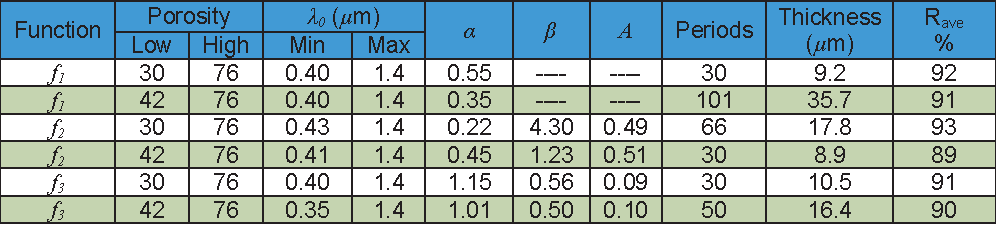
\includegraphics[width=\textwidth]
	{SITableOptimized.pdf}
\end{table}

The calculated reflectance of the optimized structures
is shown in Fig. \ref{Fig2}. it is observed that they
have an ODB in the near infrared (NIR) region of the electromagnetic spectrum, i. e.,
structures designed from functions $f_{1}$ and $f_{3}$ with a porosity contrast of
$30/76\%$ have the widest ODB spanning from 970 to 1370 nm.

\begin{figure}[tbph]
	\begin{center}
		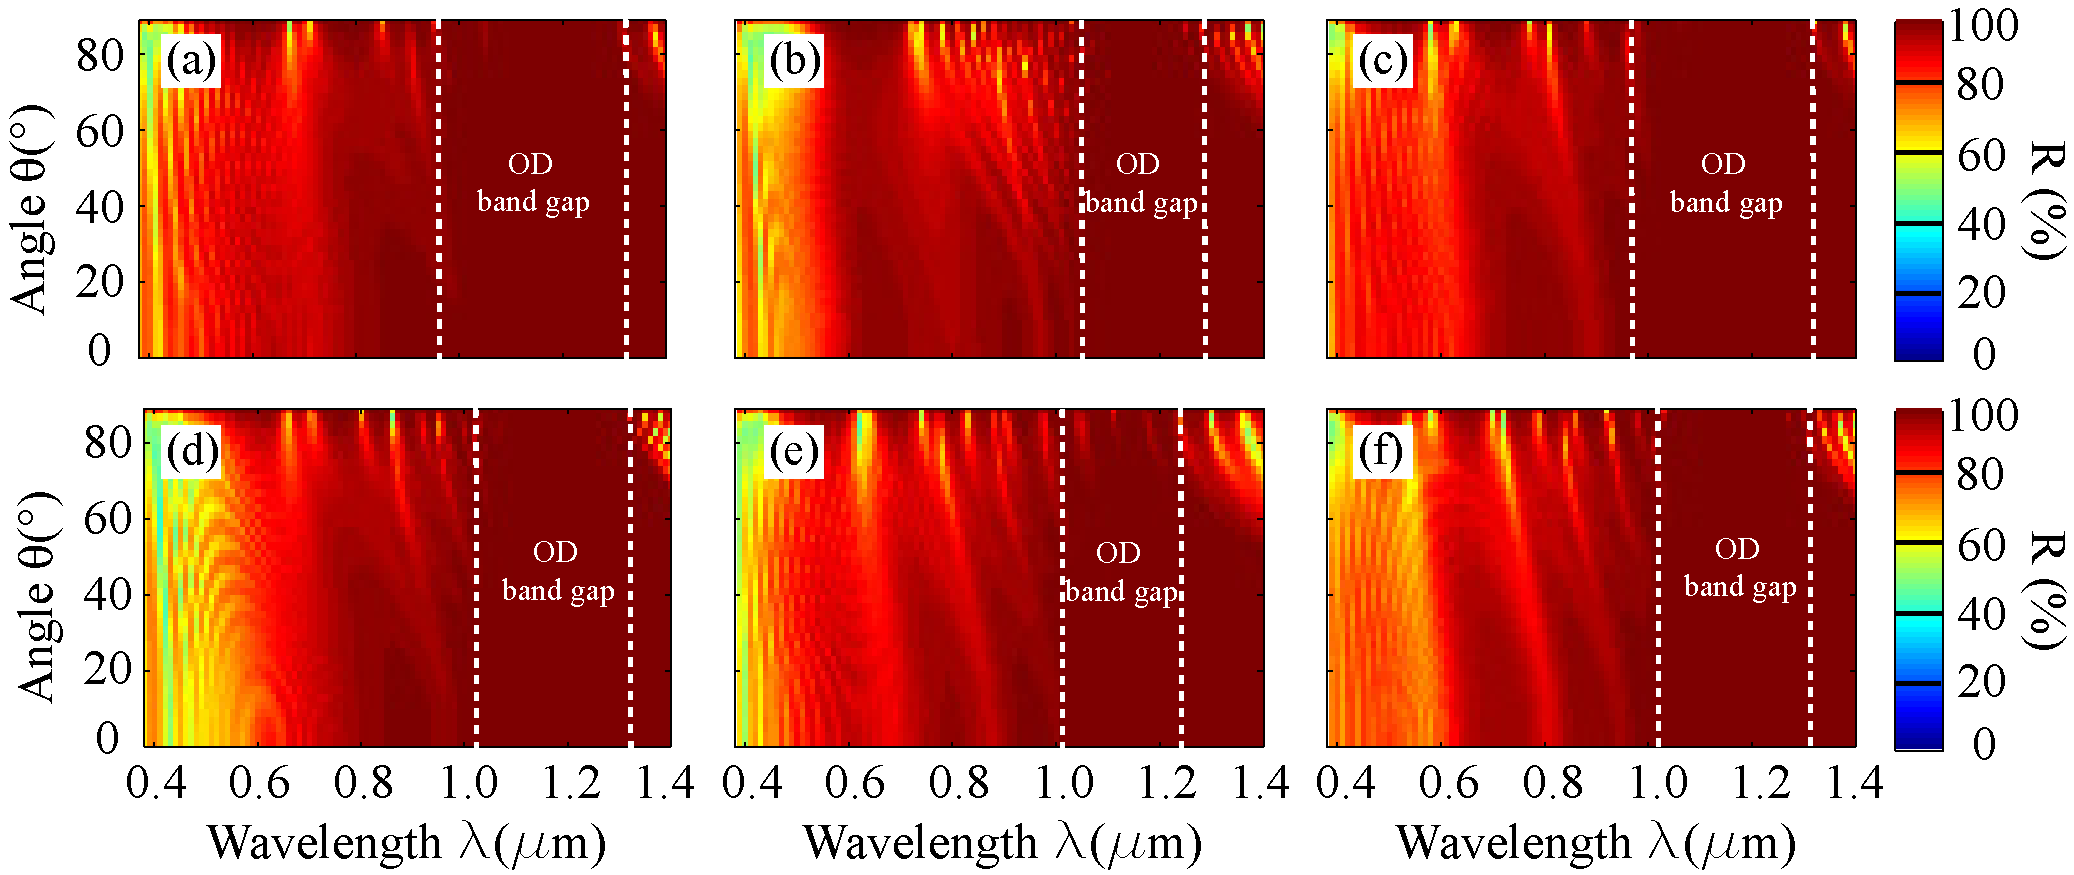
\includegraphics[width=\textwidth]
		{SIReflectanceVisNIR.pdf}
	\end{center}
	\caption{Calculated reflectance of the optimized structures
          with profile class $f_{1}$ (left), $f_{2}$
          (center) and $f_{3}$ (right) and with the porosities
          $30\%/76\%$ (upper panels) and $42\%/76\%$ (lower
          panels). The dotted lines limit the area of the ODB.}
	\label{Fig2}
\end{figure}

\newpage

\section{Photonic structure with sub-mirrors stacking}

We calclulated the trace of the transfer matrix of single Bragg mirrors formed by one period (Fig.
\ref{Fig3}(a)) and six periods (Fig. \ref{Fig3}(b)), as well as their
corresponding reflectance (Figs. \ref{Fig3}(c)
and \ref{Fig3}(d)), as a function of the design wavelength
$\lambda_{\text{dis}}$ and the wavelength of the illuminating light.
$\text{Tr}\,\bm M$ and $R(\lambda,\theta)$ were calculated for
TE polarized light incident at an angle of $45^\circ$.
Fig. \ref{Fig3}(d) shows that a
6-period mirror tuned to a  wavelength greater than 1000
nm, may also reflect in a certain region of the visible spectrum. Then, to
reinforce the reflection of the electromagnetic waves in the visible
a smaller number of periods is enough. This is another reason for increasing
number of periods in the 400 to 800 nm region.
\begin{figure}[tbph]
	\begin{center}
		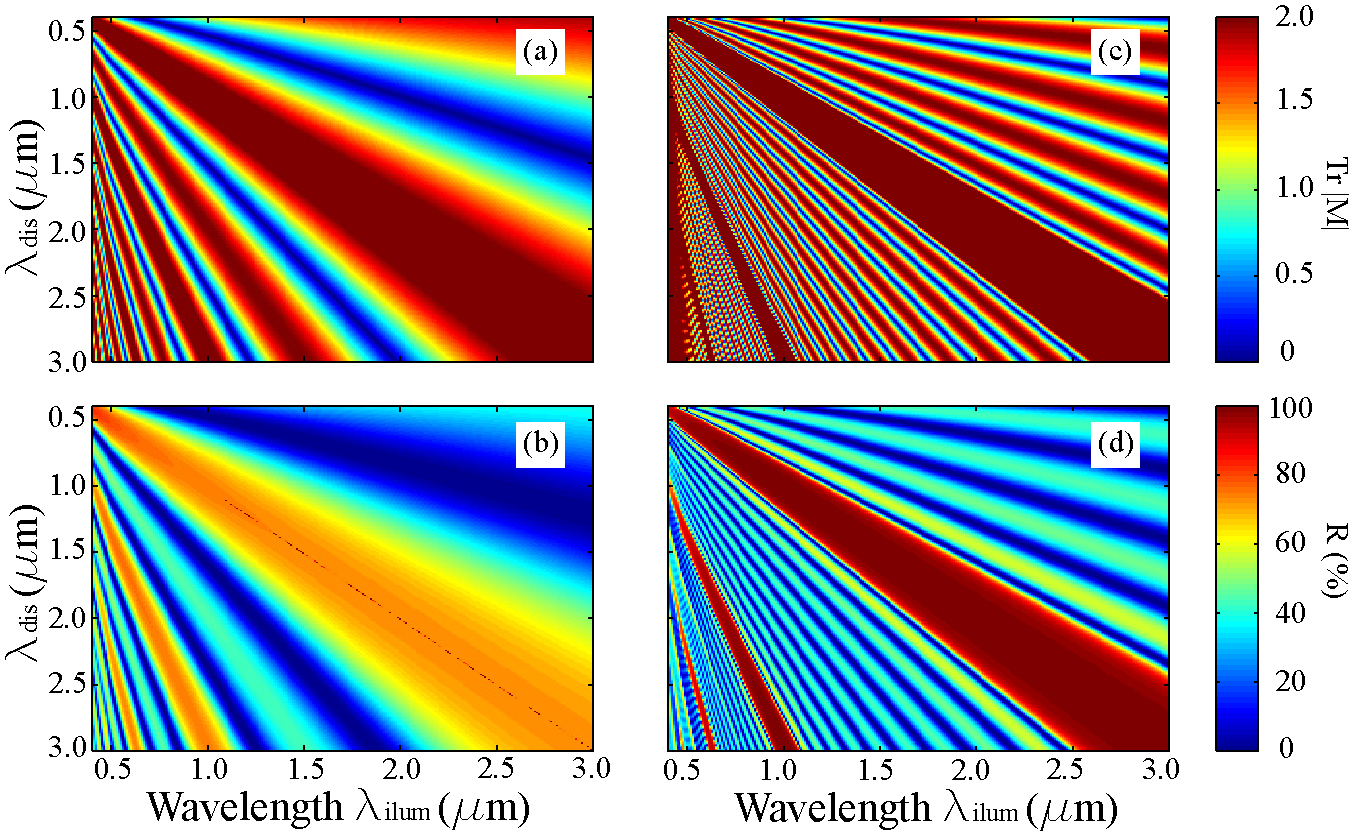
\includegraphics[width=\textwidth]
		{SITrazasyRefSE.pdf}
	\end{center}
	\caption{Calculated trace of the transfer matrix (left) and
          reflectance (right) of single Bragg mirrors one (top)
          and six (bottom) periods as a function of the design
          wavelength $\lambda_{\text{dis}}$ and the illumination
          wavelength $\lambda_{\text{ilum}}$.
          The calculations correspond to an incidence angle $\theta=45^\circ$.}
	\label{Fig3}
\end{figure}
\newpage

One strategy to design a wide band mirror could be stacking of the
sub-mirrors so that the leftmost edge of the band of one mirror begins
at the rightmost of the band of the previous mirror. However, with this
configuration, the reflectance
decreases where these band edges meet. For example, Figs. \ref{Fig4}(a)
and \ref{Fig4}(b) show the calculated $R(\lambda, \theta)$ for the structures formed
by sub-mirrors that have one and six periods, respectively, using non-polarized
light. In these cases, the calculations do not show a ODM, or quasi-ODM. For this
reason, we allowed succesive bands to overlap by some percentage
chosen to optimize the average reflectance $\braket{R}$. In Fig. \ref{Fig3}(b) of the main
article the results obtained at the end of the optimization process are shown. The
calculated $R(\lambda, \theta)$ for the structures designed with 4 periods for each
sub-mirror and using the pattern described in the main article are
shown in this document in Figs.
\ref{Fig4}(c) and \ref{Fig4}(d), respectively. Here the overlap of
the two consecutive PBGs was optimized, being $72\%$ for the first case and $78\%$
for the second. Furthermore, the calculations indicate that the structures have a
quasi-ODB.

\begin{figure}[tbph]
	\begin{center}
		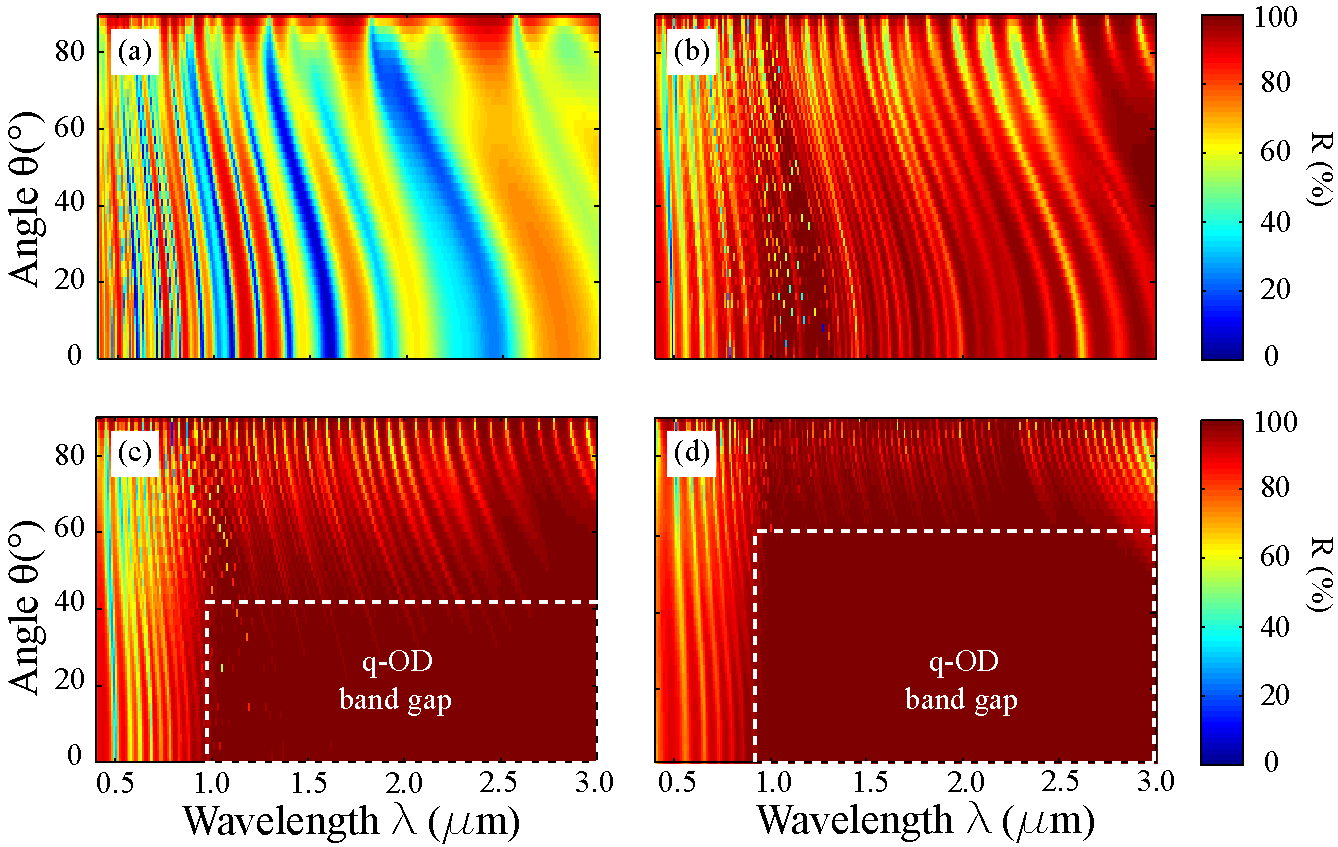
\includegraphics[width=\textwidth]
		{SIReflectanceSEoptimized.pdf}
	\end{center}
	\caption{Reflectance calculated for structures designed through the stacking of
		sub-mirrors analyzing the overlap of the PBG and the number of periods of
		each one of them. Case I: there is no overlap of the PBGs and each
		sub-mirror has (a) one period and (b) six periods. Case II: optimized
		overlap of consecutive PBGs and (c) each subsmirror has 4 periods with
		$72\%$ overlap, and (d) proposed arrangement in the main article with 6
		periods for $\lambda>800$ nm and $78\%$ overlap. The
                quasi-OD region is bounded by the dashed lines.
	}
	\label{Fig4}
\end{figure}

\end{document}
